\documentclass[a4paper,11pt]{jsarticle}

% 数式
\usepackage{amsmath,amsfonts}
\usepackage{bm}
% 画像
\usepackage[dvipdfmx]{graphicx}


\begin{document}

\title{数値解析課題}
\author{No.5 梅沢直矢}
\date{\today}
\maketitle

\section{$dy/dx=x^2-y$ 初期値$y(0)=2$について、次の問に答えなさい。}

  \subsection{オイラー法で刻み幅を$0.5$としたとして、
              $x=2$まで$y$の値を求めグラフ化しなさい。}

    \begin{figure}[h]
      \centering
      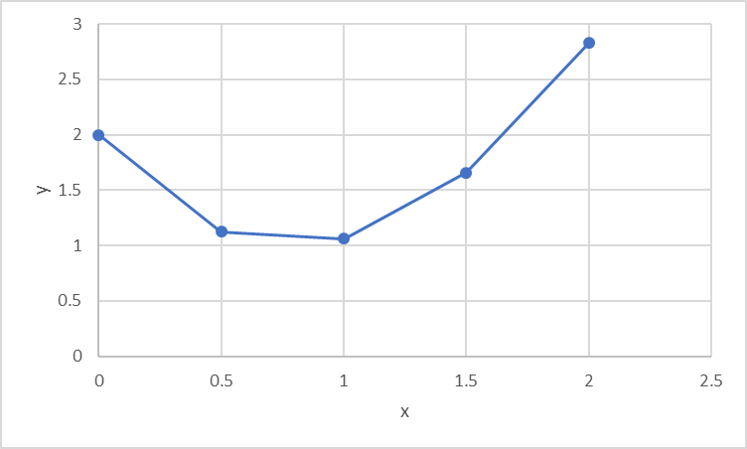
\includegraphics[scale=0.75]{1}
      \caption{$x$と$y$の値の推移}
      \label{fig:1}
    \end{figure}
                        
  \subsection{刻み幅を変え(分割数$2^n$として$n=8$まで)、
              真値($x^2-2x+2$)との誤差を検討しなさい。}
    
    \begin{figure}[h]
      \centering
      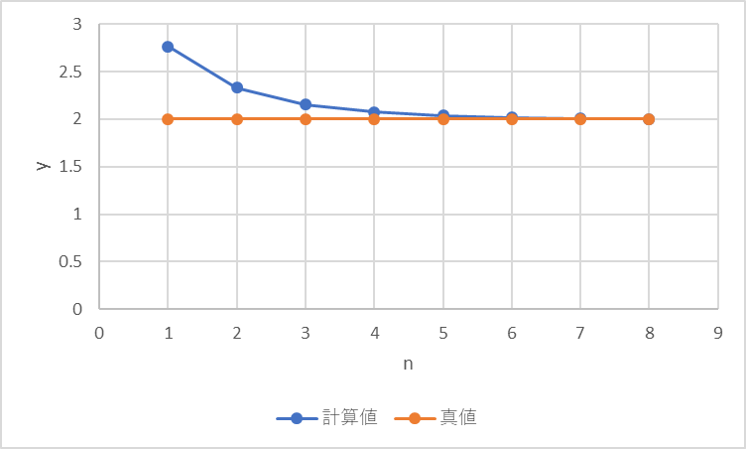
\includegraphics[scale=0.75]{2}
      \caption{計算値と真値の比較}
      \label{fig:2}
    \end{figure}

    分割数を少なくしていくと誤差が減少しているのがわかる。計算機の性能にもよるが、
    オイラー法を使うのなら、できるだけ分割数を多くしたほうがいいだろう。

  \subsection{オイラー法で誤差の出る理由を説明しなさい。}

    オイラー法は接戦を求めているため、分割数が大きくなれば
    接戦が真値に近づいていくため、精度が良くなる。そのため、
    分割数が小さいと誤差が大きくなってしまう。

  \subsection{前問の理由より、オイラー法でも誤差の出ない微分方程式を与えて、
              プログラムを実行し確かめてみなさい(刻み幅によらず誤差が出ない)。}
  
    $dy/dx=8$ 初期値$y(0)=1$

    \begin{figure}[h]
      \centering
      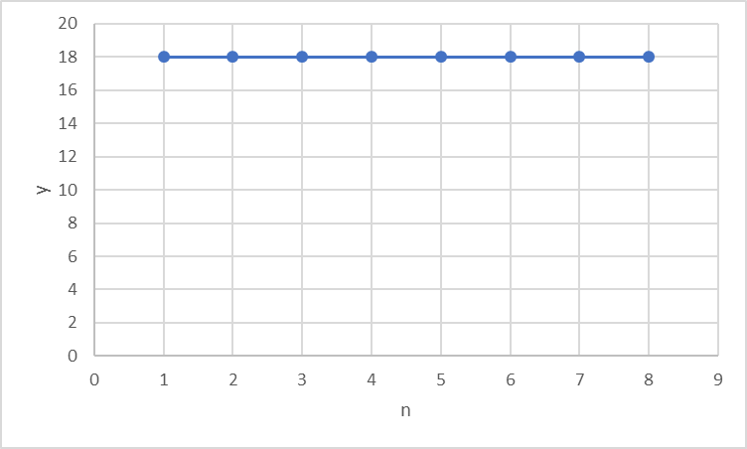
\includegraphics[scale=0.75]{4}
      \caption{刻み幅によって誤差がでない様子}
      \label{fig:4}
    \end{figure}

\section{$dy/dx=3y/(1+x)$ 初期値$y(0)=1$についてルンゲ・クッタ法を用いて
          $x$が$1$のときの$y$の値を求めなさい。このとき、
          刻み幅と解の精度について検討しなさい。}

  \begin{figure}[h]
    \centering
    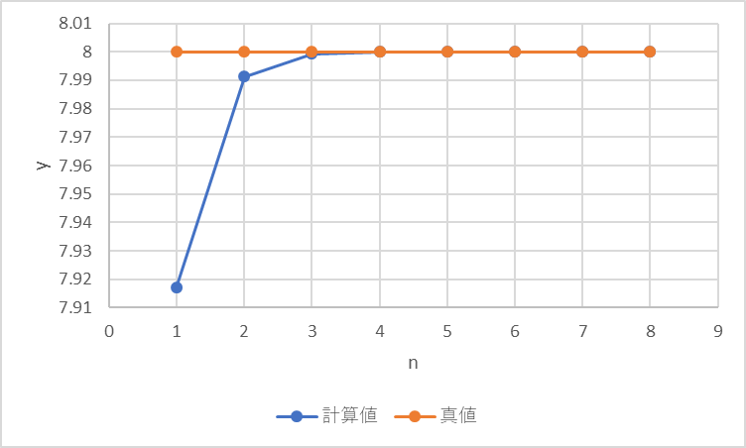
\includegraphics[scale=0.75]{5}
    \caption{刻み幅と解の推移}
    \label{fig:5}
  \end{figure}

  オイラー法と比べ、収束するまでの刻み幅が小さく、誤差もないものになっている。
        

\end{document}